\documentclass[12pt,a4paper]{report}

\usepackage{tikz}
\usepackage{amsmath}
\usepackage{listings}
\usepackage{hyperref}
\usepackage{geometry}
\geometry{margin=1in}

\title{Robotic Arm Thesis\\Actuator Subsystem Report}
\author{Your Name}
\date{\today}

\begin{document}

\maketitle

\tableofcontents

\chapter{Actuator System: Firmware Architecture and Control Algorithms}

\section{Introduction}
The actuator subsystem is implemented on an Arduino-compatible microcontroller, utilizing the Adafruit PCA9685 16-channel PWM driver for servo control. Its main function is to convert high-level trajectory commands into precise joint movements. This chapter details the firmware structure, data flow, control algorithms, calibration methods, and feedback integration, as derived directly from the provided source code.

\section{System Architecture Diagram}
Figure~\ref{fig:actuator_architecture} illustrates the actuator system architecture. The main components are: joint mapping, trajectory queue, servo driver, calibration routines, EEPROM storage, and sensor feedback.

\begin{figure}[h]
    \centering
    \begin{tikzpicture}[node distance=1.7cm,>=stealth,thick]
        % Nodes
        \node[draw,rounded corners,fill=blue!10] (serial) {Serial Interface};
        \node[draw,rounded corners,below of=serial,fill=green!10] (cmdparser) {Command Parser};
        \node[draw,rounded corners,right=3.5cm of cmdparser,fill=yellow!10] (eeprom) {EEPROM Storage};
        \node[draw,rounded corners,below of=cmdparser,fill=orange!20] (queue) {Trajectory Queue};
        \node[draw,rounded corners,below of=queue,fill=red!10] (motion) {Motion State Manager};
        \node[draw,rounded corners,left=3.5cm of motion,fill=purple!10] (calib) {Calibration \& Feedback};
        \node[draw,rounded corners,below of=motion,fill=cyan!10] (servo) {PWM Servo Driver};
        \node[draw,rounded corners,below of=servo,fill=gray!20] (joints) {Arm Joints};

        % Connections
        \draw[->] (serial) -- (cmdparser);
        \draw[->] (cmdparser) -- (queue);
        \draw[->] (cmdparser) -- (eeprom);
        \draw[->] (queue) -- (motion);
        \draw[->] (motion) -- (servo);
        \draw[->] (servo) -- (joints);
        \draw[->] (calib) -- (motion);
        \draw[->] (joints) -- (calib);
        \draw[->] (calib) -- (eeprom);

        % Labels
        \node[above of=serial,node distance=1cm] {\textbf{Actuator System Overview}};
    \end{tikzpicture}
    \caption{Actuator firmware architecture: data flow and module interconnection.}
    \label{fig:actuator_architecture}
\end{figure}

\section{Joint and Servo Configuration}
Each joint (base, right, left, twist, wrist, finger) is mapped to a servo channel. The configuration parameters (e.g., min/max pulse widths, angle values) are defined in the firmware header. Factory settings and joint limits ensure safe operation:
\begin{itemize}
    \item \textbf{Servo pulse range:} 320--2570 $\mu$s, corresponding to 0--180 degrees.
    \item \textbf{Joint channels:} BASE=0, RIGHT=1, LEFT=2, TWIST=3, WRIST=4, FINGER=5.
    \item \textbf{Factory values:} BASE = 1455 $\mu$s, RIGHT = 732 $\mu$s, etc.
\end{itemize}

\section{Firmware Main Loop Flowchart}

\begin{figure}[h]
    \centering
    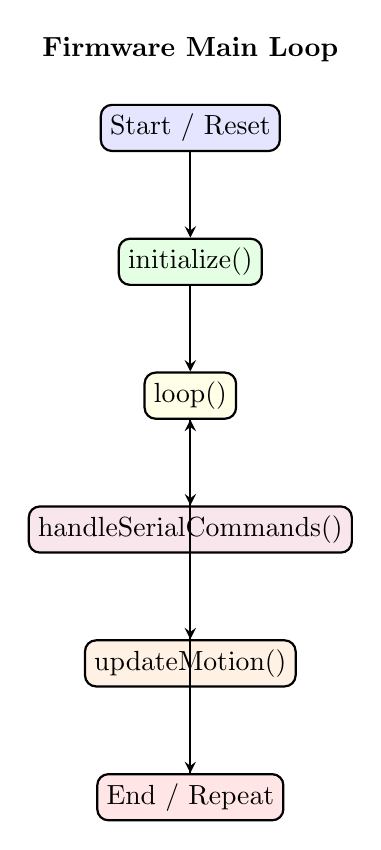
\begin{tikzpicture}[node distance=1.7cm,>=stealth,thick]
        % Nodes
        \node[draw,rounded corners,fill=blue!10] (start) {Start / Reset};
        \node[draw,rounded corners,below of=start,fill=green!10] (init) {initialize()};
        \node[draw,rounded corners,below of=init,fill=yellow!10] (loop) {loop()};
        \node[draw,rounded corners,below of=loop,fill=purple!10] (serialcmd) {handleSerialCommands()};
        \node[draw,rounded corners,below of=serialcmd,fill=orange!10] (motion) {updateMotion()};
        \node[draw,rounded corners,below of=motion,fill=red!10] (end) {End / Repeat};

        % Connections
        \draw[->] (start) -- (init);
        \draw[->] (init) -- (loop);
        \draw[->] (loop) -- (serialcmd);
        \draw[->] (serialcmd) -- (motion);
        \draw[->] (motion) -- (end);
        \draw[->] (end) -- (loop);

        % Labels
        \node[above of=start,node distance=1cm] {\textbf{Firmware Main Loop}};
    \end{tikzpicture}
    \caption{Firmware main loop: initialization, command handling, and motion update.}
    \label{fig:main_loop}
\end{figure}

\section{Trajectory Planning and Cubic Interpolation}
Trajectory motion is managed via queue structure for each joint. When a motion command is enqueued, the system computes smooth transitions using cubic polynomial interpolation.

\subsection{Cubic Trajectory Equation}
The core cubic trajectory generation function uses the following equation:
\begin{align}
\mathrm{pos}(t) = a_0 + a_1 t + a_2 t^2 + a_3 t^3
\end{align}
where coefficients are:
\begin{align*}
    a_0 &= \mathrm{startPos} \cdot 1000 \\
    a_1 &= 0 \\
    a_2 &= \frac{3 \cdot \Delta \cdot 1000000}{T^2} \\
    a_3 &= \frac{-2 \cdot \Delta \cdot 1000000000}{T^3}
\end{align*}
where $\Delta = \mathrm{endPos} - \mathrm{startPos}$ and $T$ is the total motion duration (150 ms).

\section{Actuator State Diagram (Joint Motion)}

\begin{figure}[h]
    \centering
    \begin{tikzpicture}[node distance=2.2cm,>=stealth,thick]
        % States
        \node[draw,rounded corners,fill=blue!10] (idle) {Idle};
        \node[draw,rounded corners,right=3.5cm of idle,fill=green!10] (enqueue) {Enqueue Trajectory};
        \node[draw,rounded corners,below of=enqueue,fill=yellow!10] (interpolate) {Interpolate Motion};
        \node[draw,rounded corners,below of=interpolate,fill=orange!10] (servo) {Update Servo Position};
        \node[draw,rounded corners,left=3.5cm of servo,fill=purple!10] (complete) {Motion Complete};
        \node[draw,rounded corners,above of=complete,fill=red!10] (calib) {Calibration / Feedback};

        % Connections
        \draw[->] (idle) -- node[above] {Command Received} (enqueue);
        \draw[->] (enqueue) -- (interpolate);
        \draw[->] (interpolate) -- (servo);
        \draw[->] (servo) -- node[right] {if complete} (complete);
        \draw[->] (complete) -- node[left] {next command} (enqueue);
        \draw[->] (servo) -- node[below] {if not complete} (interpolate);
        \draw[->,dashed] (calib) -- (servo);

        % Labels
        \node[above of=idle,node distance=1cm] {\textbf{Actuator State Diagram}};
    \end{tikzpicture}
    \caption{State diagram for joint motion: command, interpolation, servo update, and completion.}
    \label{fig:actuator_state_diagram}
\end{figure}

\section{Angle/Pulse Conversion Equations}

\subsection{Angle to Pulse Conversion}
\begin{equation}
\text{Pulse} = \frac{(\text{Angle} - \text{SERVO\_MIN\_SOURCE}) \cdot (\text{MaxTarget} - \text{MinTarget})}{\text{SERVO\_MAX\_SOURCE} - \text{SERVO\_MIN\_SOURCE}} + \text{MinTarget}
\end{equation}

\subsection{Pulse to Angle Conversion}
\begin{equation}
\text{Angle} = \frac{(\text{Pulse} - \text{MinTarget}) \cdot (\text{SERVO\_MAX\_SOURCE} - \text{SERVO\_MIN\_SOURCE})}{\text{MaxTarget} - \text{MinTarget}} + \text{SERVO\_MIN\_SOURCE}
\end{equation}

\section{Calibration and Feedback}
Calibration is performed in two ways:
\begin{itemize}
    \item \textbf{Manual Calibration:} User sends calibration data via serial, which is written to EEPROM.
    \item \textbf{Auto Calibration:} System moves each joint to its limit while reading sensor-trigger pins to record the travel points.
\end{itemize}
EEPROM operations ensure calibration persists across power cycles. The relevant addresses and magic values are defined for robust identification and storage.

Trigger pins (digital inputs) are mapped per joint and per limit (min/max). During auto calibration, the firmware sweeps each joint until the sensor is triggered, recording the pulse value at that point. This feedback loop ensures accurate physical limits and compensates for hardware tolerances.

\section{Robustness and Safety}
\begin{itemize}
    \item \textbf{Constraint checks:} \texttt{ConsTrain()} ensures angles/pulses stay within safe hardware limits.
    \item \textbf{Magic values:} Used in EEPROM to verify calibration data integrity.
    \item \textbf{Feedback sensors:} Minimize the risk of over-travel and hardware damage.
\end{itemize}

\section{Summary}
The actuator firmware provides a robust, scalable, and precise motion control foundation for the robotic arm. Key features include:
\begin{itemize}
    \item Modular joint and servo abstraction.
    \item Queue-based trajectory planning and cubic interpolation.
    \item Sensor feedback for calibration and safety.
    \item Persistent storage of calibration data via EEPROM.
    \item Extensible command interface for integration with vision and voice modules.
\end{itemize}
This system enables reliable and accurate manipulation essential for tasks such as pick-and-place, and sets the groundwork for higher-level autonomous control.

\begin{thebibliography}{9}
\bibitem{citation1} Arduino actuator and trajectory control principles, as implemented in ArmControl.cpp, ArmControl.h, and ArmControl.ino.
\end{thebibliography}

\end{document}
